\section{Примеры} 
\subsection{Барро-Гордон}
Положим, что матрица выигрышей двух игроков соответсвует~(\ref{table:sec:ot:real}).

$r^g= 4 $ - количество ходов совершаемое  правительством за игру\\
$r^p= 3 $ - количество ходов совершаемое  обществом за игру\\

1.
Рассмотрим случай, когда правительство скорее склонно ввести высокий уровень инфляции, а общественность предполагая, что правительство пойдет на этот шаг с высокой долей вероятности поднимет зарплаты:

$q^g =[ 0.5; 0.9; 0.7; 0.4 ]$ - соответсвующая скалярная функция \\
$q^p=[ 0.6; 0.8; 1] $ - соответсвующая скалярная функция \\

С помощью программы проведем эммуляцию 100 игр с такими исходными данными.

\begin{figure}[h]
	
	\begin{subfigure}{0.5\textwidth}
		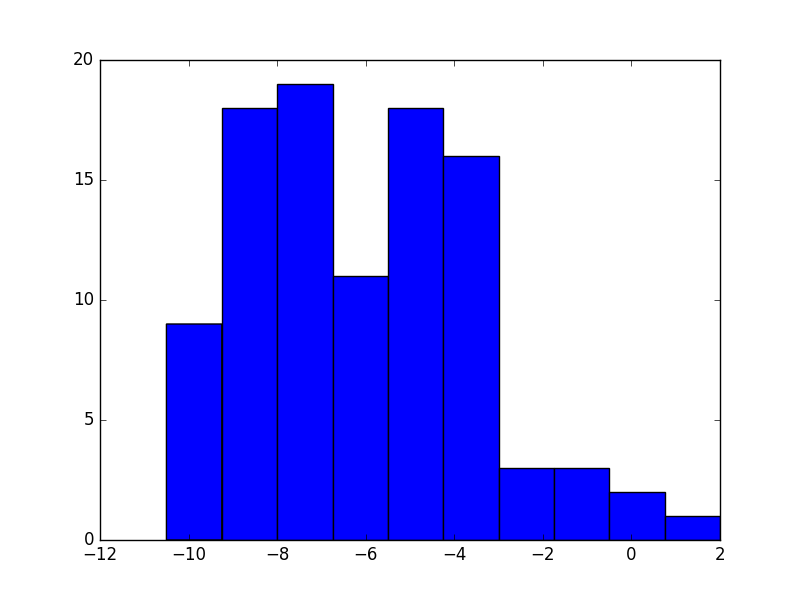
\includegraphics[width=0.9\linewidth]{Government1.png} 
		\caption{Правительство}
		\label{fig:government1}
	\end{subfigure}
	\begin{subfigure}{0.5\textwidth}
		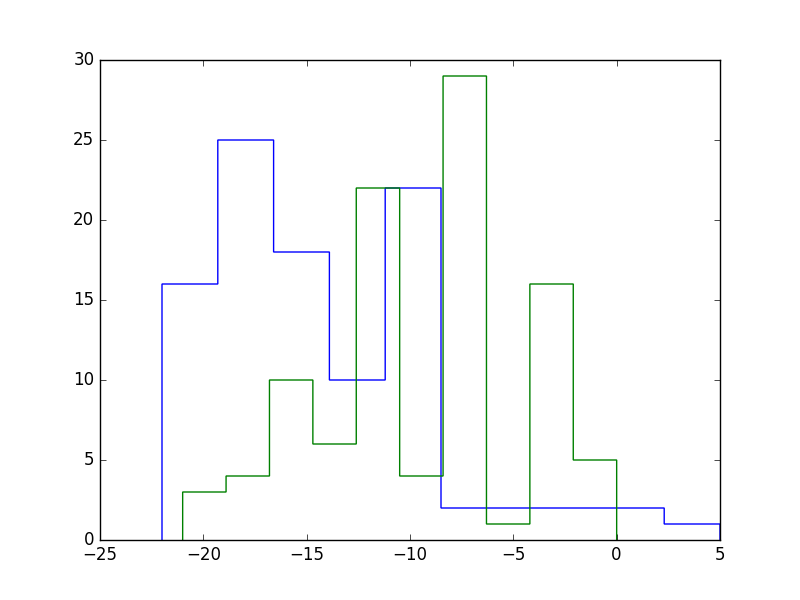
\includegraphics[width=0.9\linewidth]{Public1.png}
		\caption{Общественность}
		\label{fig:public2}
	\end{subfigure}
	
	\caption{Гистограмма выигрышей}
	\label{fig:stat1}
\end{figure}
Government's average = -6.185\\
Government's standard deviation = 2.78177551215\\
Government's asymmetry = 0.4507768484568038\\
Government's excess = -0.1516393985641198\\
Public's average = -5.47\\
Public's standard deviation = 2.76570063456\\
Public's asymmetry = 0.16025052323659267\\
Public's excess = -0.5107496427926015\\

Согалсно полученным результам легко видеть, что подобный набор стратегий невыгоден обеим сторонам, к тому же правительству из-за более "мягкого" подхода "более невыгодно".\\


2. Рассмотрим случай, когда оба игрока действут по Парето-оптмальной стратегии $(L,L)$.
\\

Для этого положим скалярные функции:\\
$q^g =[ 0; 0; 0; 0 ]$ \\
$q^p=[ 0; 0; 0] $ \\


\begin{figure}[h]
	
	\begin{subfigure}{0.5\textwidth}
		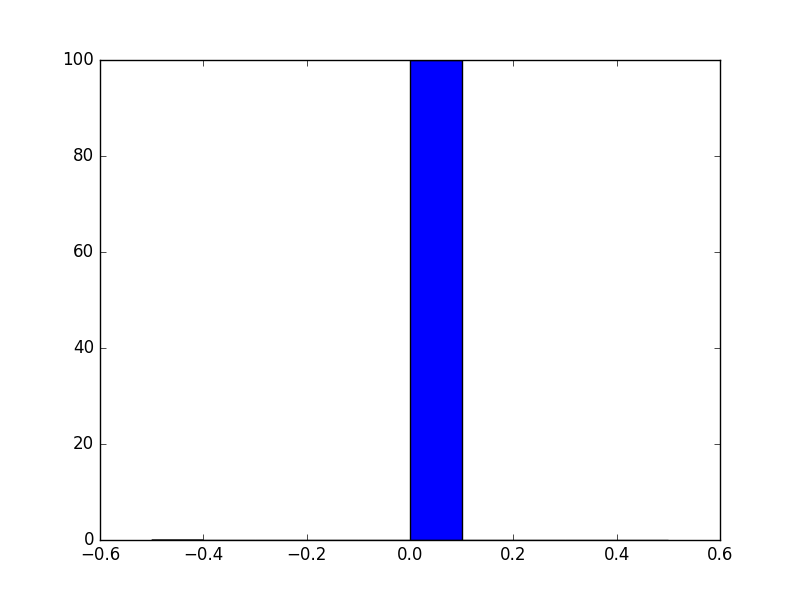
\includegraphics[width=0.9\linewidth]{Government.png} 
		\caption{Правительство}
		\label{fig:government}
	\end{subfigure}
	\begin{subfigure}{0.5\textwidth}
		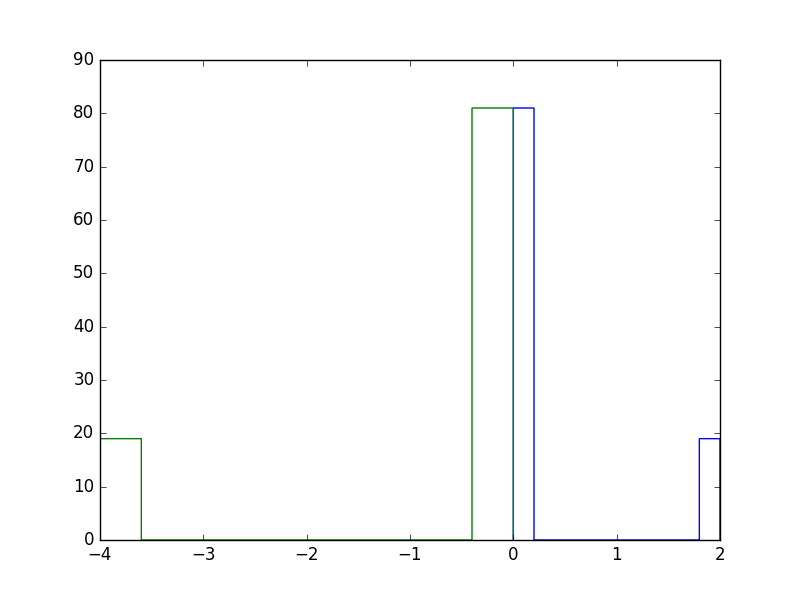
\includegraphics[width=0.9\linewidth]{Public.png}
		\caption{Общественность}
		\label{fig:public}
	\end{subfigure}
	
	\caption{Гистограмма выигрышей}
	\label{fig:stat}
\end{figure}

Government's average = 0.0\\
Government's standard deviation = 0.0\\
Government's asymmetry = 0.0\\
Government's excess = -3.0\\
Public's average = 0.0\\
Public's standard deviation = 0.0\\
Public's asymmetry = 0.0\\
Public's excess = -3.0\\

Данная стратегия является Парето-оптимальной, игрокам нет смысла отклоняться от неё. \\


3. Рассмотрим случай, когда игроки выбирают неоптимальный путь.\\
 Государство устанавливает высокий уровень инфляции, а общественность выбирает стратегию L относительно повышения зарплат.\\
	Для этого положим скалярные функции:\\
	$q^g =[ 1; 1; 1; 1 ]$ \\
	$q^p=[ 0; 0; 0] $ \\
	
	\begin{figure}[h]
		
		\begin{subfigure}{0.5\textwidth}
			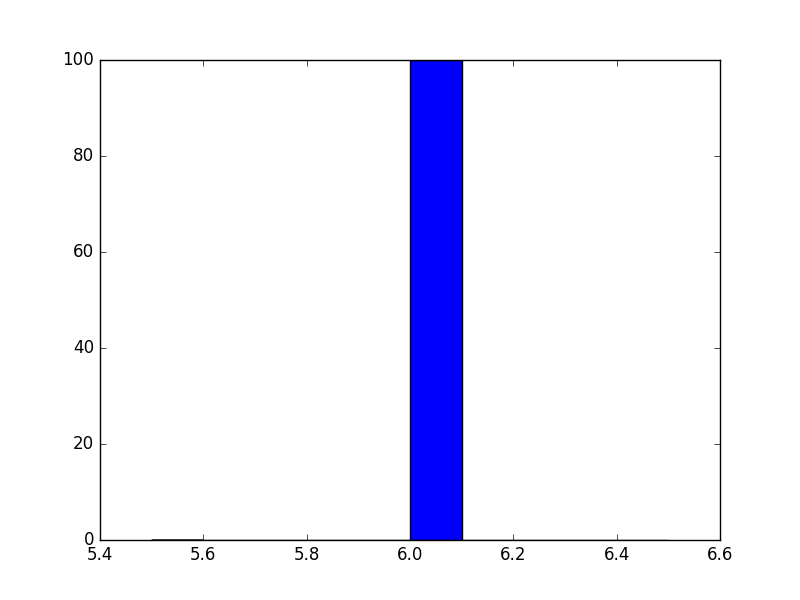
\includegraphics[width=0.9\linewidth]{Government2.png} 
			\caption{Правительство}
			\label{fig:government2}
		\end{subfigure}
		\begin{subfigure}{0.5\textwidth}
			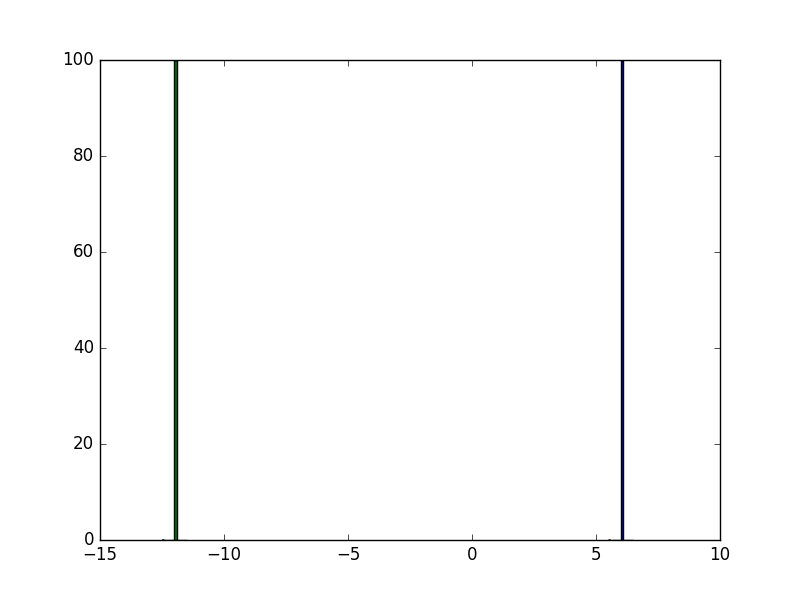
\includegraphics[width=0.9\linewidth]{Public2.png}
			\caption{Общественность}
			\label{fig:public2}
		\end{subfigure}
		
		\caption{Гистограмма выигрышей}
		\label{fig:stat2}
	\end{figure}
	
	Government's average = 6.0\\
	Government's standard deviation = 0.0\\
	Government's asymmetry = 0.0\\
	Government's excess = -3.0\\
	Public's average = -12.0\\
	Public's standard deviation = 0.0\\
	Public's asymmetry = 0.0\\
	Public's excess = -3.0\\
	
	
Как можно увидеть данная ситуация выгодная правительству, однако совершенно противоречит интересам общественности. Ссылаясь на  классическую модель Барро-Гордона отметим, что данная стратегия на краткосрочную перспективу. Следовательно разумному правительству данная стратегия является неприемлимой на долгосрочную перспективу.\\


4. Рассмотрим обратную ситуацию, когда правительство решает не повышать уровень инфляции, а общественность повышает уровень зарплат.\\
	 	Для этого положим скалярные функции:\\
	 	$q^g =[ 0; 0; 0; 0 ]$ \\
	 	$q^p=[ 1; 1; 1] $ \\
 
 	\begin{figure}[h]
 		
 		\begin{subfigure}{0.5\textwidth}
 			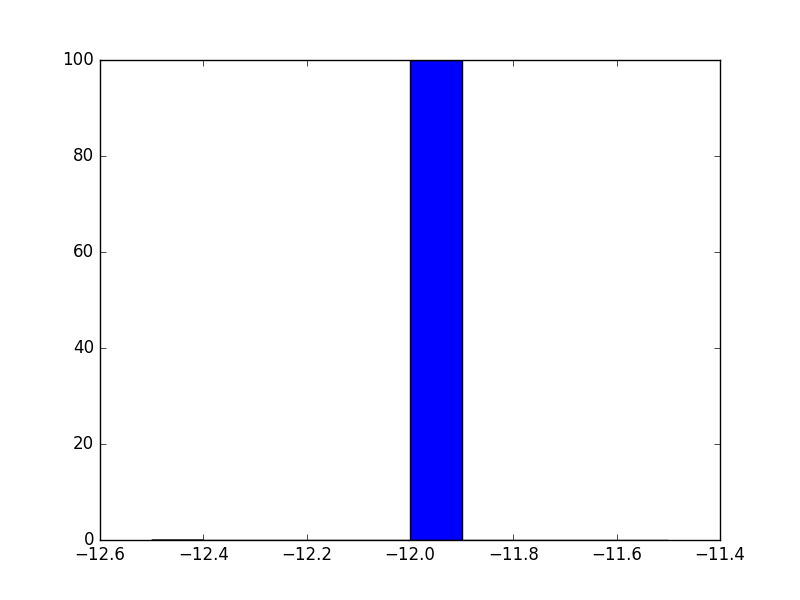
\includegraphics[width=0.9\linewidth]{Government3.png} 
 			\caption{Правительство}
 			\label{fig:government3}
 		\end{subfigure}
 		\begin{subfigure}{0.5\textwidth}
 			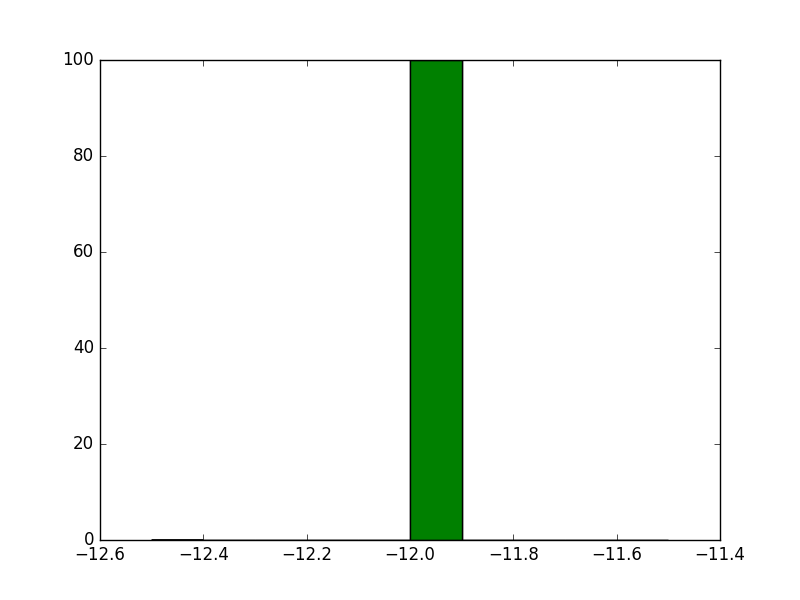
\includegraphics[width=0.9\linewidth]{Public3.png}
 			\caption{Общественность}
 			\label{fig:public3}
 		\end{subfigure}
 		
 		\caption{Гистограмма выигрышей}
 		\label{fig:stat3}
 	\end{figure}
 Government's average = -12.0\\
 Government's standard deviation = 0.0\\
 Government's asymmetry = 0.0\\
 Government's excess = -3.0\\
 Public's average = -12.0\\
 Public's standard deviation = 0.0\\
 Public's asymmetry = 0.0\\
 Public's excess = -3.0\\
 
 Данная стратегия является равносильно невыгодной для обоих игроков.\\
 
 5. Рассмотрим выбор стратегии, которая является равновесием по Нэшу $(H,H)$\\
 Для этого положим скалярные функции:\\
 $q^g =[ 1; 1; 1; 1 ]$ \\
 $q^p=[ 1; 1; 1] $ \\
 
 	\begin{figure}[h]
 		
 		\begin{subfigure}{0.5\textwidth}
 			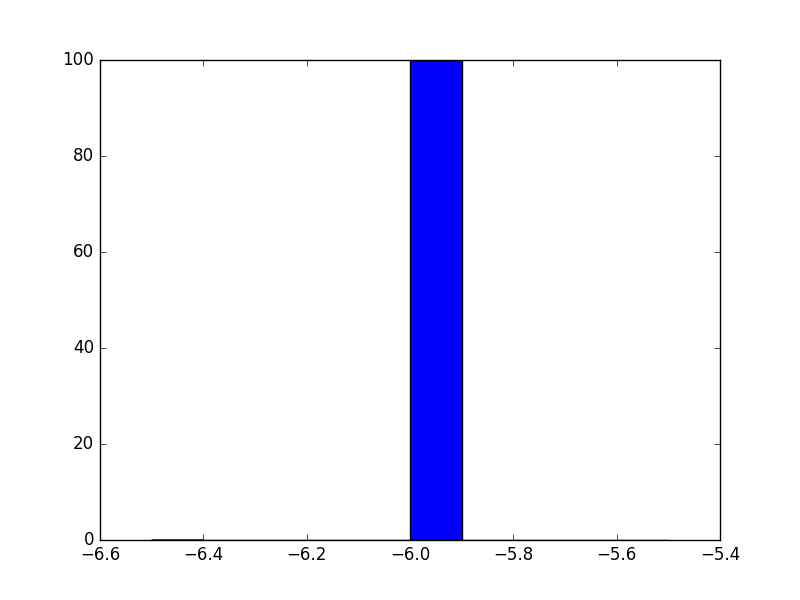
\includegraphics[width=0.9\linewidth]{Government4.png} 
 			\caption{Правительство}
 			\label{fig:government4}
 		\end{subfigure}
 		\begin{subfigure}{0.5\textwidth}
 			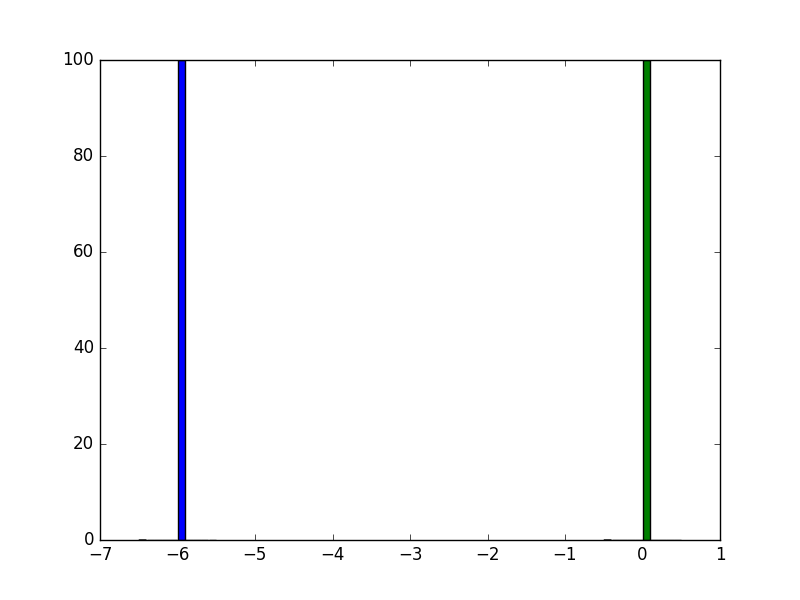
\includegraphics[width=0.9\linewidth]{Public4.png}
 			\caption{Общественность}
 			\label{fig:public4}
 		\end{subfigure}
 		
 		\caption{Гистограмма выигрышей}
 		\label{fig:stat4}
 	\end{figure}
 	Government's average = -6.0\\
 	Government's standard deviation = 0.0\\
 	Government's asymmetry = 0.0\\
 	Government's excess = -3.0\\
 	Public's average = 0.0\\
 	Public's standard deviation = 0.0\\
 	Public's asymmetry = 0.0\\
 	Public's excess = -3.0\\
 	
 Стратегия хоть и является равновесием по Нэшу, тем не менее не Парето-оптимальна.\\
 
 
 	
Империческим путем мы подтвердили правдивость теории. 


\subsection{Монополия профсоюза}
